% Metódy inžinierskej práce

\documentclass[10pt,twoside,slovak,a4paper]{article}
%\usepackage{multirow}
\usepackage[slovak]{babel}
\usepackage{pdfpages}
%\usepackage[T1]{fontenc}
\usepackage[IL2]{fontenc} % lepšia sadzba písmena Ľ než v T1
\usepackage[utf8]{inputenc}
\usepackage{graphicx}
\usepackage{url} % príkaz \url na formátovanie URL
\usepackage{hyperref} % odkazy v texte budú aktívne (pri niektorých triedach dokumentov spôsobuje posun textu)

\usepackage{cite}
%\usepackage{times}

\pagestyle{headings}

\title{Tvorba softvéru pomocou umelej inteligencie
\thanks{Semestrálny projekt v predmete Metódy inžinierskej práce, ak. rok 2021/22, vedenie: Ing. Vladimír Mlynarovič}} % meno a priezvisko vyučujúceho na cvičeniach

\author{Ľubomír Novotný\\[2pt]
	{\small Slovenská technická univerzita v Bratislave}\\
	{\small Fakulta informatiky a informačných technológií}\\
	{\small \texttt{xnovotnyl1@stuba.sk}}
	}

\date{\small 1. október 2021} % upravte



\begin{document}

\maketitle

\begin{abstract}

 Tento článok sa zaoberá využitím umelej inteligencie pri testovaní softvéru, a najmä používateľského rozhrania. Používateľské rozhranie testované softvérom riadeným udalosťami (event driven software testing) môže ťažiť z využitia AI riešení. Umelá inteligencia výrazne pomohla procesu automatizácie rôznych softvérových procesov. Riešenia pomocou umelej inteligencie znižujú cenu a garantujú lepšiu kvalitu a dôkladné testovanie. Testovanie používateľského rozhrania sa môže pokladať za najnáročnejšiu časť testovania softvéru. Hoci výsledky sú dosť predbežné, ale aplikovanie rôznych AI techník pre testovanie používateľského rozhrania preukázalo prínos ideálnych výsledkov. Pri tvorbe a udržiavaní softvéru nám umelá inteligencia môže podstatne pomôcť.\\\\
 \textbf{Kľúčové slová:} testovanie softvéru, umelá inteligencia, AI, grafické používateľské rozhranie, GUI
\end{abstract}

\section{Úvod}

Umelá inteligencia je nový prelom v oblasti informatiky~\ref{AI}. Umelá inteligencia má veľký vplyv v posledných rokoch na postupy pri riešení problémov, ale aj na naše každodenné životy. AI používa počítače na riešenie inak neriešiteľných problémov a zlepšenie kvality dočasných počítačových systémov. Dôležitou otázkou je, či môžeme priamo použiť AI na problémy softvérového inžinierstva~\ref{SWE}, a či procesy softvérového inžinierstva sú schopné využiť umelú inteligenciu~\ref{pouzitie AI pri SW}.
Testovanie a podobné aktivity si vyžadujú veľa pozornosti počas celej fázy tvorby softvéru, aby sme mohli vytvoriť požadovaný softvér. Na tento zdĺhavý a komplikovaný problém môžeme použiť umelú inteligenciu.  Umelá inteligencia je schopná vykonávať širokú škálu činností, ktorú by inak nebolo možné naprogramovať konvenčným spôsobom. Testovanie používateľského rozhrania je podobné rôznym iným činnostiam, ktoré sme dokázali vyriešiť pomocou umelej inteligencie. V posledných rokoch boli možnosti umelej inteligencie vyšetrované, a boli použité na automatizáciu testovania softvéru.

\subsection{Softvérové inžinierstvo} \label{SWE}
 Softvérové inžinierstvo \cite{swemb} sa zaoberá tvorbou softvérových systémov ale aj efektivitou softvérových systémov. Efektivita je dôležitá, pretože v reálnom svete máme na vývoj a údržbu ohraničené zdroje, stanovené požiadavky a časový limit. Preto môžeme povedať, že softvérové inžinierstvo sa zaoberá tvorbou väčších softvérových systémov, čo najefektívnejším spôsobom. Pri tvorbe sa sústreďujeme na tvorbu čo najspoľahlivejšieho softvéru, pričom sa snažíme čo najlepšie využiť schopnosti softvérových inžinierov.
Tvorbu softvéru môžeme realizovať rôznymi spôsobmi. Všetky procesy tvorby softvéru sa vykonávajú v jednotlivých etapách. Tie môžeme nazvať aj ako životný cyklus softvéru. Poznáme viacero takýchto modelov alebo životných cyklusov, ktorými sa môžeme riadiť pri tvorbe softvéru \cite{swebp}:
\begin{itemize}
    \item \textbf{Vodopádový model} je založený na jednoznačnom vymedzení činností, ktoré na seba nadväzujú a neprelínajú sa. Je vymedzená postupnosť krokov, ktoré  za sebou nasledujú. Po poslednom kroku máme náš projekt dokončený.
    \item \textbf{Agilný model} je protikladom vodopádového modelu. Uplatňuje sa v projektoch v ktorých je jasný cieľ, ale nedokážeme presne určiť detailný plán projektu bez priebežných prototypov. Agilný model je interaktívny, pružný a prírastkový. Je závislý na častej spätnej väzbe počas procesu tvorby  prototypovania. Nastavujeme si stále nové požiadavky a parametre na základe a skúseností z jednotlivých iterácií. 
\end{itemize}
\begin{center}
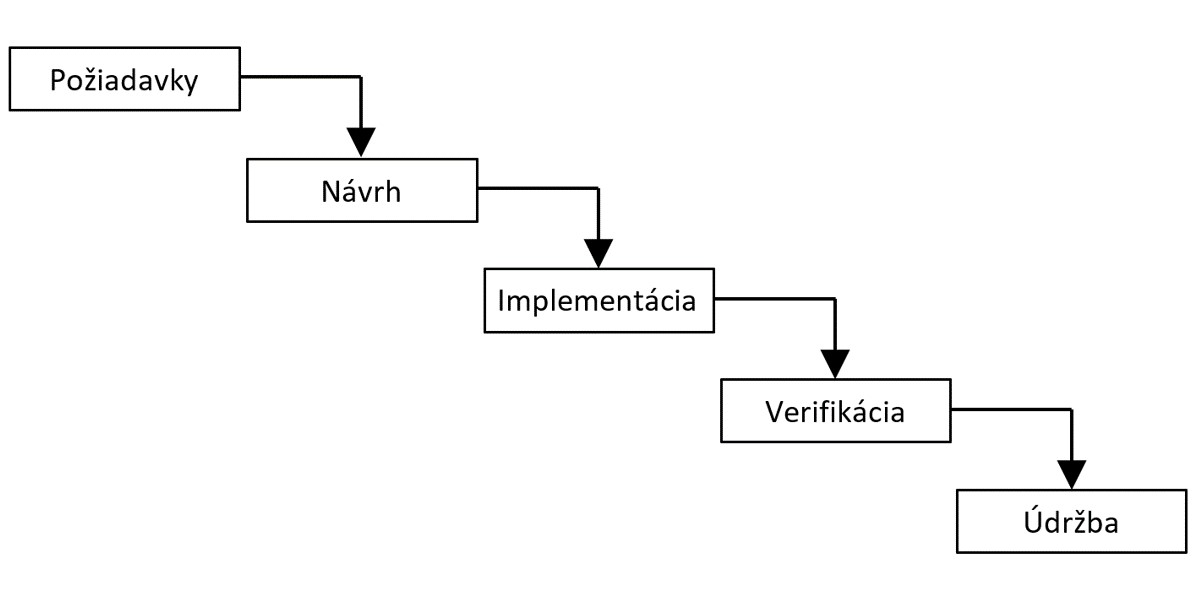
\includegraphics[scale=0.4]{vodopad1}
\end{center}
\begin{center}
Obr. 1 Vodopádový model tvorby softvéru podľa \cite{swebp}.
\end{center}


\subsection{Testovanie softvéru} \label{testovanie}
 Podľa \cite{swemb}: "testovateľnosť je úsilie, ktoré treba vynaložiť na testovanie vlastností výrobku, napr. či vykazuje požadované správanie." Testovanie programu \cite{CSEroadmap} začína už na začiatku vývoja, keď samotní programátori testujú funkčnosť počas programovania. Konečné testovanie časti softvéru, by nemal vykonávať tvorca softvéru, a malo by sa vykonávať systematicky, aby sa testovaním podrobila čo najväčšia časť programu. Testovanie je pomerne zložitá ale dôležitá oblasť, preto sa testovaniu venuje odborník, a nie programátor.
Pri samotnom procese testovania sa softvéroví inžinieri sústreďujú na celý životný cyklus testovania, ktorý začína testovaním funkcií a končí preberacím testovaním a zahŕňa \cite{testovanie}:
\begin{itemize}
	\item Testy funkcií a modulov - vykonávané prevažne softvérovými inžiniermi počas implementácie.
	\item Integračné testy - testovanie viacerých modulov súčasne.
	\item Alfa a beta testovanie - testovanie systému v prostredí skutočnej prevádzky. 
    \item Validačné testovanie - overovanie splnení špecifických požiadavok určených zákazníkom.
    \item Preberacie testovanie - posledné testovanie pred odovzdaním produktu.
\end{itemize}

\begin{center}
   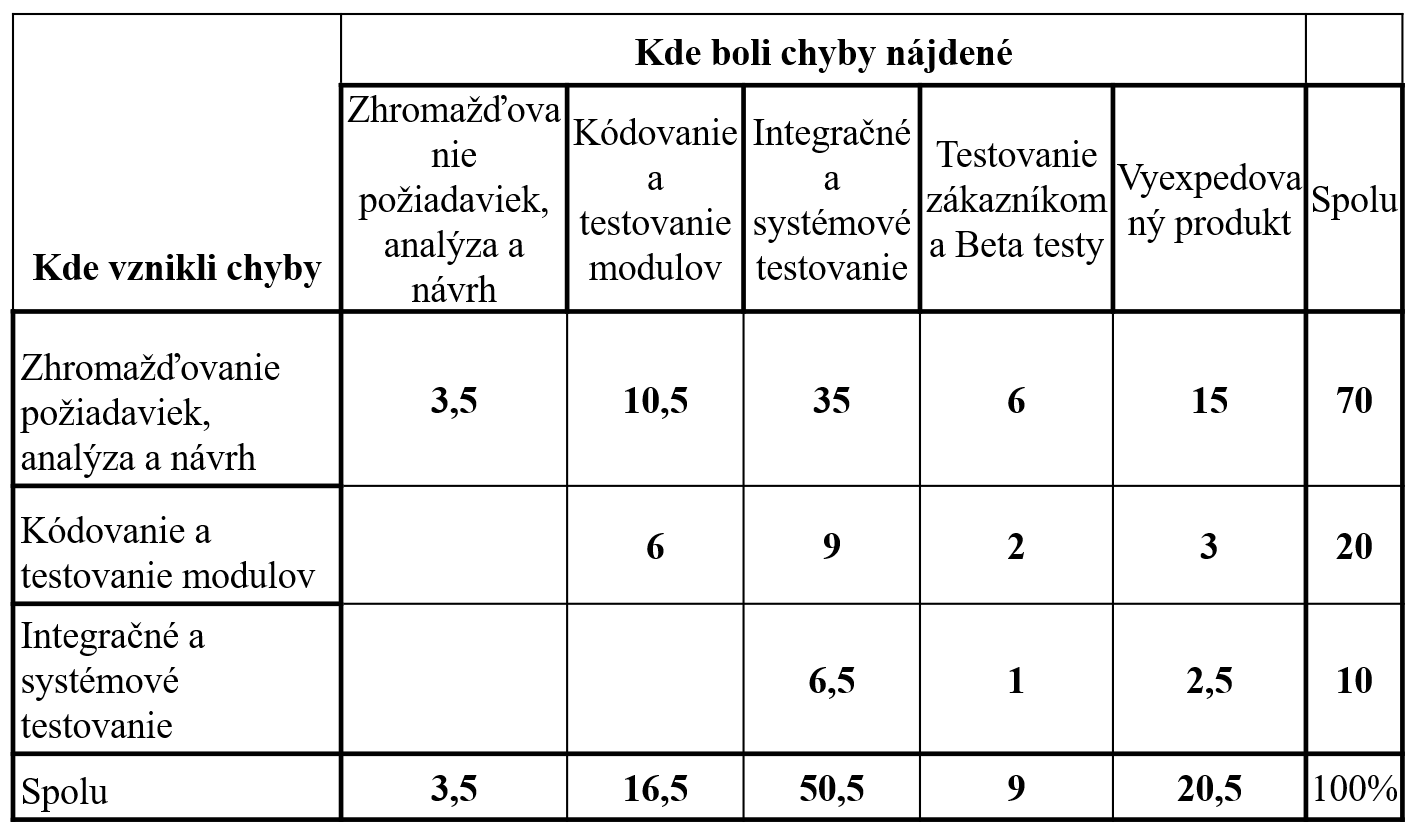
\includegraphics[scale=0.4]{tabulka.png} 
\end{center}
\begin{center}
    Obr. 2 Tabuľka rozloženia chýb a ich objavenia počas vývoja aplikácie podľa \cite{testovanie}.
\end{center}

 Chyby môžu vzniknúť v každom štádiu vývoja aplikácie \cite{testovanie}, vrátane testovania. Vodopádový spôsob vývoja softvéru \cite{CSEroadmap} sa spolieha na testovanie softvéru až po dokončení dizajnu, kódovania a splnenia podmienok. Agilný a iteratívny prístup tvorby softvéru predstavili prototypovanie, ktoré je použité na overenie požiadavok a verifikáciu minulej iterácie. Neustála verifikácia sa snaží využiť formálne metódy a inšpekcie počas procesu tvorby, na rozdiel od testovacej fázy na konci vývojovej fázy.
\subsection{Umelá inteligencia}\label{AI}

 Pod umelou inteligenciou (AI) chápeme softvér, ktorý napodobňuje ľudské kognitívne funkcie tým, že má schopnosť učiť sa a riešiť problémy. Program sa správa tak, že ak by to robil človek, považovali by sme ho za inteligentného. Okrem rozpoznávania reči, obrazov, prekladu do jazykov dokáže imitovať rozmýšľanie ľudí - učiť sa, uvažovať, riešiť problémy, sám hľadať spôsoby, ako sa dostať k cieľu. Je to aj schopnosť počítačov používať algoritmus na učenie sa z dát a získané vedomosti použiť na rozhodovanie podobné ľudskému. Umelá inteligencia ako celok stavia vo veľkej miere na základoch mnohých ďalších vedných odborov, a to predovšetkým na informatike, matematike, štatistike, logike, lingvistike či neurovedách. Podobnosť umelej a ľudskej inteligencie je ale iba povrchná a nie je správne ich stotožňovať.\cite{AIvMed}

\section{Používanie AI pri tvorbe a testovaní SW} \label{pouzitie AI pri SW}

 Umelá Inteligencia môže byť použitá pri vývoji a testovaní nového softvéru, alebo jeho údržbe. Použitie umelej inteligencie má veľa výhod \cite{6926420}:
\begin{itemize}
	\item Zredukovanie cyklov tvorby softvéru a testovania, umožňujúc priniesť produkt na trh rýchlejšie.  
	\item Vyššia efektivita testov, plné využitie hardvérových zdrojov. 
	\item Šetrenie na pracovnej sile, zníženie počtu ľudí podieľajúcich sa na teste a znížiť cenu testovania.
    \item Vyššia stabilita a efektivita testu a testovacieho procesu.
    \item Zlepšenie presnosti a precíznosti testu, zvýšenie dôveryhodnosti v softvér.
    \item Softvérové testovacie nástroje sú relatívne jednoduché a môžu priniesť kvalitnejšie výsledky.
    \item Úlohy ktoré nie je možné vykonať ručne, ale môže to urobiť automatizované testovanie, ako je testovanie záťaže a výkonu.
\end{itemize}
Za súčasných okolností, automatické testovanie softvéru nedokáže vyriešiť všetky problémy. Automatické testovanie softvéru má nasledujúce obmedzenia a problémy \cite{6926420}:
\begin{itemize}
	\item Nedokáže nahradiť manuálne testovanie.
	\item Manuálne testovanie nachádza viacero defektov ako automatizované testovanie.
	\item Manuálne testovanie je vysoko závislé od kvality testu.
	\item Automatizácia testu môže obmedziť vývoj softvéru.
	\item Samotný nástroj nemá imagináciu, nedokáže sa snažiť nájsť chyby ako človek.
\end{itemize}

\subsection{Rola AI v testovaní softvéru} \label{rola ai v sw}

Rôzne nástroje AI sa používajú na generovanie testovacích údajov , výskum vhodnosti údajov, optimalizáciu a analýzu pokrytia, ako aj správu testov. Na účely testovania softvéru sa použilo mnoho ďalších techník založených na AI \cite{6926420}.
ABC (Artificial Bee Colony Optimization) \cite{7542311} je optimalizačný algoritmus založený na inteligentnom správaní sa včelieho roja pri hľadaní potravy. ABC algoritmus sa zameriava na miesta v kóde, kde je definovaná alebo použitá premenná, ktorá predstavuje zdroj potravy. V modeli sa kolónia skladá z troch skupín včiel: zamestnaných včiel, pozorovateľov a prieskumníkov. Predpokladá sa, že pre každý zdroj potravy existuje len jedna umelo zamestnaná včela. Zamestnané včely idú k svojmu zdroju potravy a tancujú na tejto ploche. Zamestnaná včela, ktorej zdroj potravy bol opustený, sa stane prieskumníkom a začne hľadať nový zdroj potravy. Pozorovatelia sledujú tance zamestnaných včiel a vyberajú si zdroje potravy v závislosti od tancov. Vybraný zdroj sa následne otestuje vygenerovanými vstupnými údajmi. Testovanie modelom ABC dosahuje v porovnaní s inými technikami takmer globálnu optimalizáciu s niekoľkými vykonanými testami.

\subsection{Rola AI v testovaní GUI} \label{rola ai v gui}

Grafické používateľské rozhrania (GUI) sú jedným z najpotrebnejších prvkov v dnešnom vývoji softvéru. Priebeh testovania GUI aplikácie si vyžaduje obrovské úsilie kvôli zložitosti týchto aplikácií. GUI môže mať aj v malej aplikácii problém obrovského počtu stavov, pretože sa môže generovať príliš veľa testovacích prípadov. Testovanie zahŕňa vypracovanie súboru úloh, vykonanie týchto úloh a porovnanie skutočných výsledkov s očakávanými výsledkami. Technika zahŕňa detekciu reakcie aplikácie na udalosti myši a klávesnice, komponentov, ako sú tlačidlá, lišty ponúk, obrázky, lišty nástrojov, textové polia, reakcie na vstup používateľa atď. Testovanie GUI sa môže vykonávať manuálne aj automatizovane, pričom obe metódy majú svoje výhody a nevýhody \cite{6926420}. Techniky na automatizované testovanie zahŕňajú generovanie GUI na základe modelu, generovanie testov na základe modelu a automatizáciu generovania testovacích prípadov, aby bolo možné automaticky regenerovať testy pri každej zmene GUI, ktoré modelujú správanie používateľského rozhrania. Mnoho činností v testovaní GUI je potrebné automatizovať, aby boli dané postupy ekonomicky vhodné. V optimálnom prístupe sa použijú inteligentný vyhľadávací agenti (Intelligent Search Agent) (ISA) pre optimálne generovanie testovacej sekvencie a inteligentný agent na optimalizáciu testovacích prípadov (Intelligent Test Case Optimization Agent) (ITOA) pre optimálne generovanie testovacích prípadov.\cite{6926420}

\section{Reakcia na témy} \label{reakcie}
\paragraph{Spoločenské súvislosti.}
V dnešnej dobe si musíme uvedomiť, ako veľmi je náš svet závislý od výpočtovej technológie. Od obyčajného prehliadania internetu, až po dôležité ekonomické a bezpečnostné úlohy každej krajiny. Chyba v systéme banky môže znamenať, že sa ľudia nedostanú k svojim peniazom, alebo neočakávané správanie softvéru burzy môže vytvoriť ekonomickú depresiu. Preto je testovanie správnosti funkcie daných programov dôležite pre správne fungovanie  našej spoločnosti. V posledných rokoch môžeme zaznamenať trend okupovania sa elektronikou. Takzvaný IOT (internet of things) začína vstupovať do našich životov a do našich domovov. Inteligentný asistenti, inteligentné osvetlenie a mnoho ďalších technológií sa dostalo do našich domovov za účelom lepšej kontroly a starania sa o náš domov. Správnosť týchto zariadení je každým dňom dôležitejšia, keďže ich prítomnosť sa neustále zväčšuje.
\paragraph{Historické súvislosti.}
Vývoj softvéru sa počas histórie informatiky menil. Od samotných programovacích jazykov, písania kódu, funkcionalite programov, až po samotné prístroje pre ktorý bol softvér tvorený. Každá zmena v tomto prostredí nám pomohla tvoriť lepšie a rýchlejšie programy a aplikácie. Jednou z týchto zmien bolo to, ako testujeme softvér. Softvér je citlivý na každý vonkajší a vnútorný atribút od spôsobu, ako  je naprogramovaný, až po zariadenie na ktorom má vykonávať jeho danú činnosť. Donedávna testovanie prebiehalo pomerne konzervatívne. Programátor vyberie časť kódu, a testuje na ňom rôzne vstupy, alebo manuálne testuje používateľské rozhranie, ktoré sa testuje veľmi neefektívne. Postupom času sa pohľad na testovanie zmenil. Začali sa generovať vstupné údaje, používanie softvérov na testovanie, čím sa šetrilo na pracovnej sile, zdĺhavé testovanie sa prenieslo na počítač, aplikovanie rôznych algoritmov na optimalizáciu testov, neskôr sa začala používať aj umelá inteligencia atď. Hoci stále existujú chyby, ktoré nájde len človek, inovácie v testovaní nám taktiež pomohli pri tvorbe softvéru.
\paragraph{Technológia a ľudia.}
Pri vývoji softvéru programátori neustále kontrolujú ich vlastný kód. Je priam nemožné napísať kód bez chýb, ktoré si programátor neuvedomil pri jeho tvorbe. Preto sa kód neustále testuje celým jeho vývojom, aj po tom, čo už bol dokončený a proces tvorby softvéru sa posunul na inú fázu. Počas písania kódu programátor strávi veľa svojho času hľadaním chýb v kóde, čo je vysoko neefektívne, stojí to veľa nákladov, ale aj psychickej sily samotného programátora. Chyby v kóde sú niekedy také závažné, že viacero programátorov sa musí sústrediť na nájdenie a opravenie chyby v kóde. Zapojenie nástrojov ktoré pomôžu programátorom pri vývoji softvéru sa zefektívni postup a zlepšia sa pracovné podmienky pre programátorov, ktorí môžu vytvoriť lepší produkt pre ľudí, ktorý ho budú používať.
\paragraph{Udržateľnosť a etika.}
Po vytvorení aplikácie alebo daného softvéru sa práca programátorov nekončí. Väčšina softvérov má po vystavení na trh určitú dobu údržby, v ktorej je daný softvér podporovaný spoločnosťou, ktorá ho vytvorila. Podpora softvéru zahŕňa najmä bezpečnosť softvéru, stabilitu, prípadne aj nové funkcionality. Spomenuté spôsoby testovania môžu pomôcť nie len pri vývoji, ale aj pri údržbe softvéru a jeho častí, pretože pri každej aktualizácií sa softvér musí znova testovať. Často sa chyby objavia aj na miestach, kde v predošlých verziách neboli, preto testovanie pri údržbe softvéru by nemalo byť podcenené a limitované len na zmenené časti softvéru. Lepšie testovacie nástroje nám môžu pomôcť udržiavať softvér s menšími nákladmi, čo by sa malo pozitívne odzrkadliť na dnešnom a budúcom softvéri.

\section{Záver} \label{zaver}

Testovanie je prítomné v každej fáze tvorby softvéru, aj preto je veľmi nákladné a časovo náročné. Hľadať možné zlepšenia a inovácie v tomto smere má teda rozhodne zmysel. Použitie techník AI a rôznych algoritmov sa ukázalo byť vhodným prostriedkom pre vývoj a testovanie softvéru a teda aj GUI. Hoci automatické testovanie softvéru pomocou rôznych nástrojov má aj svoje nevýhody a slabé stránky, vývoj softvéru bude prosperovať pri zavedení týchto nástrojov a techník. Môžeme ho aplikovať v mnohých častiach vývoja, kde zlepšuje kvalitu testovania nášho softvéru. Techniky testovania softvéru obohatené o AI a algoritmy by určite mali byť zahrnuté do procesu testovania.

% týmto sa generuje zoznam literatúry z obsahu súboru literatura.bib podľa toho, na čo sa v článku odkazujete
\bibliography{literatura}
\bibliographystyle{plain} 
\end{document}
